\chapter{Experiments and Results}

The main aim of this section is to assess the use of static features when involved in the characterization of Android malware and benignware samples used to train detection tools. Thus, through
the use of several machine learning classifiers, it is studied if this combination with stacking methods is feasible and, if
so, to assess its performance when applied to build a machine learning aided Android malware
detection tools.

\section{1st Stage training experiments} \label{1ststagetrain}

For the 1st stage training step of our model, the selected ensemble classifiers were run with the Scikit-learn library for Python\cite{scikitlearn}.
They include AdaBoost, XGBoost, Catboost, Bagging Classifier, K-nearest neighbors, Neural network, Random Forest. 
All these ensemble classifiers were tested with the previously mentioned dataset through a 10-folds cross validation with the accuracy scoring method shown below.

$$Accuracy = (TP+TN)/(TP+TN+FP+FN)$$
$$where: TP = \text{True positive}; FP = \text{False positive};$$$$TN = \text{True negative}; FN = \text{False negative}$$

For a better evaluation of the capacity of these algorithms to extract
and generalize conclusions, several experiments were conducted to judge the individual performance of all models.
The results are shown in Table \ref{table:1ststage} and Figure \ref{fig:1ststage}

\begin{table}[htbp]
    \centering
    \caption{Experiments results on 1st training stage}
    \label{table:1ststage}
    \begin{adjustbox}{width=\textwidth}
        
    \begin{tabular}{|cccccccc|}
        \hline
        
        \textbf{Model} & \textbf{Activities CV} & \textbf{API calls CV} & \textbf{Opcodes CV} & \textbf{Permissions CV} & \textbf{Receivers CV} & \textbf{Services CV} & \textbf{System CV} \\ \hline
        LightGtextbf & 0.5094 & 0.8783 & 0.8519 & 0.7979 & 0.8486 & 0.5094 & 0.7866 \\ \hline
        Bagging & 0.5108 & \textbf{0.8817} & 0.8544 & 0.8094 & 0.8577 & 0.5099 & 0.7986 \\ \hline
        CatBoost & 0.5103 & 0.8762 & 0.8499 & 0.8048 & 0.8525 & 0.5031 & 0.7912 \\ \hline
        Neural Network & 0.5124 & 0.8518 & 0.8189 & 0.7841 & 0.8429 & 0.5092 & 0.7692 \\ \hline
        XGBoost & 0.5099 & 0.8740 & 0.8469 & 0.8008 & 0.8388 & 0.5094 & 0.7809 \\ \hline
        Random Forest & 0.5098 & 0.8238 & 0.8348 & 0.6143 & 0.7946 & 0.5064 & 0.7526 \\ \hline
        K-Neighbors & 0.5050 & 0.8466 & 0.8279 & 0.7817 & 0.8440 & 0.5116 & 0.7743 \\ \hline
        
        \end{tabular}

    \end{adjustbox}
    \end{table}

    \begin{figure}[htbp]
        \centering
        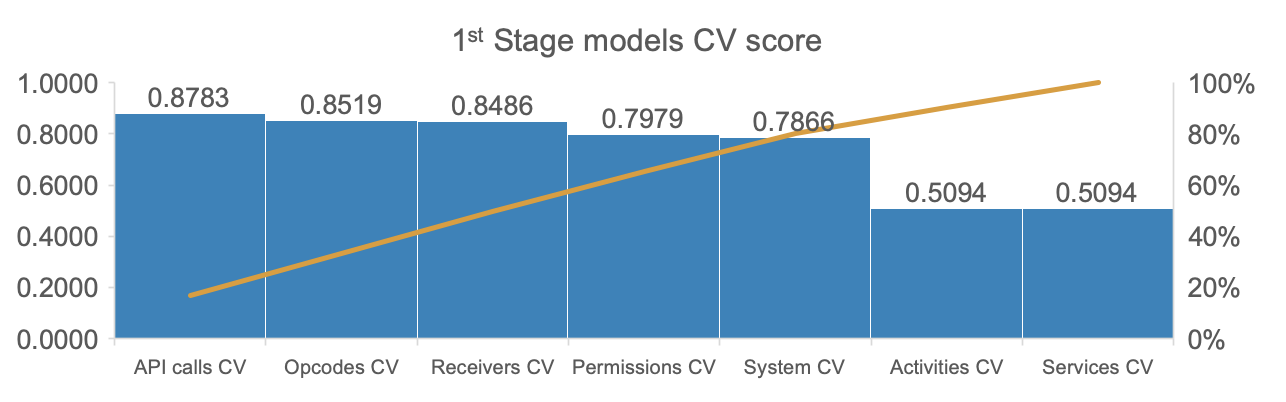
\includegraphics[width=\textwidth]{./Figure/1ststage.png}
        \caption{1st Stage models CV accuracy score average}
        \label{fig:1ststage}
      \end{figure}

 In particular, API
calls compose the most appropriate representation to build a machine learning classification
tool, exhibiting a 88.17\verb+%+ accuracy with a Bagging classifier. In general,
this algorithm obtains the best results overall.
% It is remarkable the fact that a combination of API calls with other also competitive features,
% such as opcodes or receivers, which have proved to be powerful at building detection mechanisms, does not lead to better values.

It is remarkable the fact that not only API calls have good results but also Opcodes and Receivers have proved to be powerful at building detection mechanisms as we can see in Figure \ref{fig:1ststage}. 

Other conclusions can be made after the analysis of these results. In the case of services and activities, it can be seen how these features do not allow to discern the nature of the
sample, since they provide very high-level information unable to describe specific behaviors.

\section{2nd Stage training experiments}

In the 2nd stage for training, we used the predictions results of the 1st stage as input to training our 4 selected classifiers. Due to we have only 49 inputs to each model, we selected 4 algorithms that are good to handle with small datasets. It is Neural Network, Logistic Regression Classifier, Linear SVC, Random Forest.
All these classifiers were tested with the previously mentioned dataset through a 10-folds cross validation with accuracy scoring method as section \ref{1ststagetrain}.
The results are shown in the Table \ref{table:2ndstage} and Figure \ref{fig:2ndstage}.


\begin{table}[htbp]
    \centering
    \caption{Experiments results on 2nd training stage}
    \label{table:2ndstage}
        
        \begin{tabular}{|cc|}
            \hline
            
            \textbf{Model} & \textbf{CV score} \\ \hline
            \textbf{LinearSVC} & \textbf{0.9356} \\ \hline
            \textbf{RandomForestClassifier} & \textbf{0.9339} \\ \hline
            \textbf{Neural Network} & \textbf{0.9334} \\ \hline
            \textbf{LogisticRegression} & \textbf{0.9312} \\ \hline
            1st Stage best model & 0.8817 \\ \hline
            
            \end{tabular}
    \end{table}

    \begin{figure}[htbp]
        \centering
        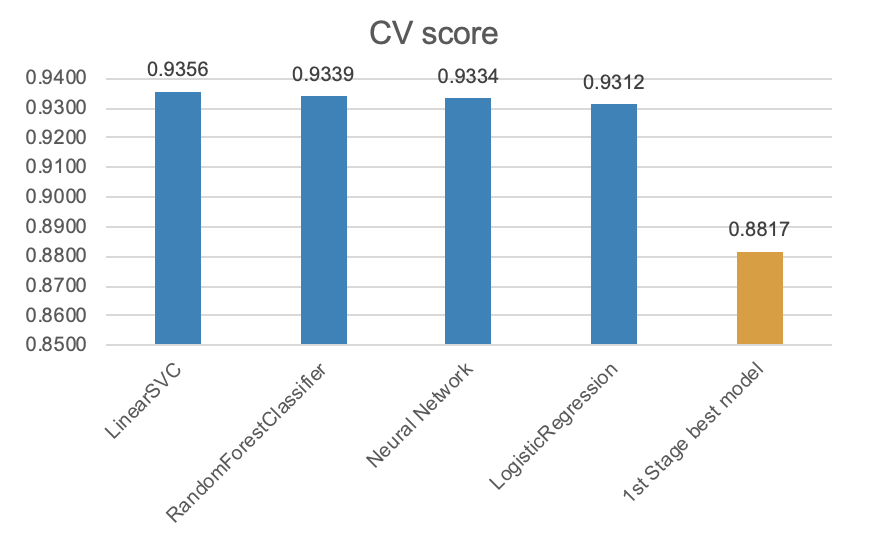
\includegraphics[scale=0.7]{./Figure/2ndstage.png}
        \caption{2nd Stage models CV accuracy score}
        \label{fig:2ndstage}
      \end{figure}

From these results from the 2nd stage, we could see that our all models score are better than the best score from the 1st stage. Moreover, comparing to the best model at this stage we have a difference of about 5.39\verb+%+ from the 1st stage best model. This fact could prove that our Stacking method is a useful and very powerful method to improve the performance of malware detection systems or models.

\section{3rd Stage training experiments}

In the 3rd stage, we use the 4 outputs from the 2nd stage to do our final prediction.
Also, we tested the same algorithms of the 2nd stage to find out the best model. The validation method and dataset are the same as the previous stages.
The results are shown in Table \ref{table:3rdstage} and Figure \ref{fig:3rdstage}.

\begin{table}[htbp]
    \centering
    \caption{Experiments results on 3rd training stage}
    \label{table:3rdstage}
        
        \begin{tabular}{|cc|}
            \hline
            
            Model & CV score \\ \hline
            LinearSVC & 0.9213 \\ \hline
            RandomForestClassifier & 0.9209 \\ \hline
            Neural Network & 0.9205 \\ \hline
            LogisticRegression & 0.9203 \\ \hline
            \textbf{1st Stage best model} & \textbf{0.9356} \\ \hline
            
            \end{tabular}
    \end{table}

    \begin{figure}[htbp]
        \centering
        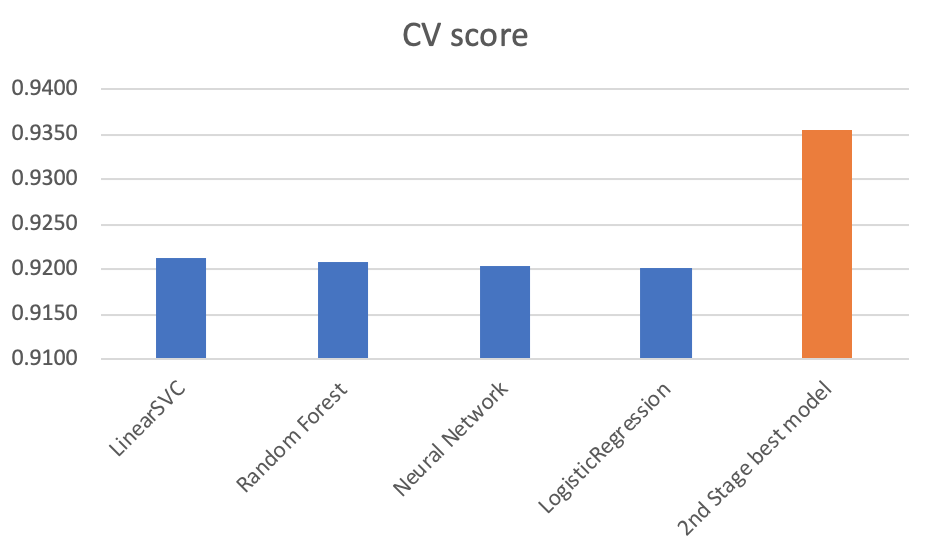
\includegraphics[scale=0.6]{./Figure/3rdstage.png}
        \caption{3rd Stage models CV accuracy score}
        \label{fig:3rdstage}
      \end{figure}

From these results, we can see that the 3rd stage models could not improve the accuracy score from the 2nd stage best model score. And the difference in the score of our 3rd stage models is only 0.1\verb+%+. It may happen because the size of our input for the 3rd stage was very small, only 4 inputs. So we have a conclusion that stacking many steps in small data may cause poor performance in classification models.


\section{Comparing to other techniques}

In this section, we compare the results of our experiments to other static analysis techniques to detect Android malware. We can see in Table \ref{table:comparison} related works results with different datasets.


\begin{table}[htbp]
    \centering
    \caption{Comparison of android malware static analysis techiniques}
    \label{table:comparison}
    \begin{adjustbox}{width=\textwidth}
    \begin{tabular}{|l|m{40mm}|m{40mm}|l|}
        \hline
        
        Paper & Input & Dataset & Accuracy score \\ \hline
        Samaneh et al. \cite{samaneh}& Intents, Permissions & 114 apps (Malware 57, Benign-ware 57) & 98\% \\ \hline
        Manzhi et al.\cite{manzhi} & Resource file, Manifest file, executable class dex files. & 1,100 apps (Malware 550, Benign-ware 550) & 98.1\% \\ \hline
        Zi Wang et al.\cite{ziwang} & Permissions, API function calls & 6334 apps (Malware 4000, Benign-ware 2334) & 93\% \\ \hline
        Zarni et al.\cite{zarni} & Permissions & 500 apps & Around 91\% \\ \hline
        Xiong et al.\cite{xiong} & Permissions & 540 apps (Malware 298, Benign-ware 342) & More than 90\% \\ \hline
        \textbf{Our proposed system} & \textbf{APK}(Activities, API function calls, Opcodes, Permissions, Receivers, Services, System) & \textbf{20,000 apps (Malware 10,000, Benign-ware 10,000)} & \textbf{94\%} \\ \hline
        
        \end{tabular}
    \end{adjustbox}
    \end{table}

